% This is samplepaper.tex, modified for the LLM Bias Traffic Light Tool Paper
\documentclass[runningheads]{llncs}
%
\usepackage[T1]{fontenc}
\usepackage{graphicx}
\usepackage{amsmath}
\usepackage{amssymb}
\usepackage{booktabs} % For professional tables
\usepackage{xcolor}

\begin{document}
\author{Soheyb Boutadjine\inst{1}\orcidID{0009-0007-4382-5554} \and
Luiza Corpaci\inst{1}\orcidID{0009-0004-4432-6843} \and \\
Ludwig Kampel\inst{1}\orcidID{0000-0002-1870-5143}}
%
\authorrunning{S. Boutadjine et al.}
%
\institute{AAAM Research, Association for Advancing Applications of
Mathematics,\\ Vienna, Austria,
\url{https://www.aaam.info/}
\\
\email{\{sboutadjine,luiza,lkampel\}@aaam.info}}
%
\title{LLM Bias Traffic Light: A Local, Real-Time Browser Extension for Auditing Algorithmic Fairness}
\titlerunning{LLM Bias Traffic Light}

\maketitle              % typeset the header of the contribution
%
\begin{abstract} 
As Large Language Models (LLMs) reshape how people access information, concerns regarding their tendency to introduce and amplify social biases such as those related to age, nationality, socioeconomic status, amongst others have intensified. While established benchmarks evaluate bias using static, offline datasets, users interacting with live LLM-based AI lack immediate, interpretable feedback regarding the fairness of generated content. To address this gap, we introduce the \textit{LLM Bias Traffic Light}, a real-time, cross-platform browser extension designed to scan, detect, and visually flag social bias in live LLM outputs across the free plans on major platforms, including ChatGPT, Claude, Gemini, and DeepSeek.

Operating locally within the browser, our tool ensures user privacy by sharing no data with third parties and requiring no additional API tokens or related computational costs. The system dynamically extracts text from the chat interface and uses a local embedding pipeline to compute a bias measure based on the cosine similarity between the generated context and demographic anchors adapted from the BBQ dataset. 

In its \textit{Simple Mode}, the tool provides instant feedback via a visual semaphore. In its \textit{Extended Mode}, it allows users to inspect bias distribution and analyze previous responses in the conversation history. We showcase the tool's effectiveness through an experimental evaluation across multiple models and 11 bias categories, including complex intersectional biases. By turning  embedding-based metrics into immediate visual feedback, the tool supports more critical and transparent interactions with generative AI.

\keywords{Large Language Models (LLMs) \and Bias Detection \and Real-time Evaluation \and Algorithmic Fairness \and Sentence Embeddings \and Browser Plugin \and Trustworthy AI.}
\end{abstract}


\section{Introduction}

The rapid proliferation of Large Language Models (LLMs) across critical sectors, including healthcare, education, and software engineering, has raised significant ethical concerns regarding the societal harms and biases they may perpetuate \cite{parrish-etal-2022-bbq,satheesh2025gg,huang2025code}. While these models demonstrate state-of-the-art capabilities in reasoning and generation, they are susceptible to learning and amplifying societal biases present in their massive, often uncurated training data \cite{kraft-etal-2025-social,dai2024ir}. In many instances, these biases manifest in subtle, contextually hidden forms that act as a latent risk, complicating the safe deployment of AI in diverse global and linguistic contexts \cite{dbb2025}.

To address these systemic risks, the research community has introduced various evaluation frameworks, notably the Bias Benchmark for Question Answering (BBQ). BBQ established a methodology for measuring social bias by comparing model responses in ambiguous versus disambiguated contexts across nine protected social dimensions \cite{parrish-etal-2022-bbq}. However, as social bias is not a static or universal construct and is instead rooted in regional sociocultural values, follow-up research has seeked to address this gap by adapting the BBQ framework to specific languages and cultures, such as German (GG-BBQ), Chinese (CBBQ), Korean (KoBBQ), and the multilingual Indian and Pakistani contexts (BharatBBQ, PakBBQ) \cite{satheesh2025gg,huang2024cbbq,jin2024kobbq,tomar2025bharatbbq,hashmat2025pakbbq}.

Despite this progress, several critical challenges persist. Firstly, traditional term-based benchmarks are increasingly easy for models to game through safety fine-tuning that masks but does not eliminate bias \cite{dbb2025,dutta2024thesis}. Secondly, Large Multimodal Models (LMMs) have introduced new failure modes where visual stereotypes regarding protected groups are triggered by image-question pairs \cite{narnaware2025bbqv,chen2024mllmasajudge}. Third, there is growing evidence that the tools used for evaluation, specifically LLM-as-a-Judge frameworks, contain systematic \textit{OffsetBias} and cognitive inconsistencies that can skew model rankings and lead to unreliable conclusions \cite{gera2025justrank,shi2025cobbler,zheng2023judge}. Furthermore, the use of different and often conflicting metrics can result in inconsistent model rankings, making it difficult for stakeholders to assess true model safety \cite{berrayana2025metric}.

In this paper, we propose the \textbf{LLM Bias Traffic Light} framework, a standardized and intuitive diagnostic tool for visualizing bias risks on English text. By synthesizing foundational benchmarks with modern methodological advancements, including adversarial bias elicitation, the Traffic Light system categorizes model behavior into safe (Green), cautionary (Yellow), and high-risk (Red) zones \cite{cantini2025clear,siska-etal-2024-examining}. Our framework offers a comprehensive diagnostic approach that accounts for regional nuances and evaluation robustness, enabling more reliable and culturally aware deployment of foundation models worldwide.

The rest of the paper is structured as follows. Section~\ref{sec:related} reviews related work on bias benchmarking and embedding-based fairness metrics. Section~\ref{sec:data} describes the BBQ dataset underlying our anchor construction and scoring pipeline. Section~\ref{sec:design} presents the technical design of the bias scoring mechanism, including the Traffic Light classification logic. Section~\ref{sec:architecture} details the system architecture and data flow of the browser extension. Section~\ref{sec:eval} reports our experimental evaluation across four LLMs and 11 bias categories. Section~\ref{sec:threats-validity} discusses the threats to validity of our approach. Section~\ref{sec:future} outlines directions for future work, and Section~\ref{sec:conclusions} concludes the paper.


\section{Related Work}
\label{sec:related}

The systematic quantification of social bias is a multi-disciplinary challenge that has evolved from human-centric diagnostic tools in the social sciences, such as the Implicit Association Test (IAT), to statistical fairness metrics in classical machine learning. In the latter domain, bias is traditionally operationalized through measures of statistical parity or equalized odds across demographic groups. However, the shift toward Large Language Models (LLMs) has rendered these structured data methodologies insufficient, necessitating new frameworks capable of auditing unstructured and high-dimensional semantic outputs.

Current LLM bias research relies heavily on standardized benchmarks, most notably the Bias Benchmark for Question Answering (BBQ) \cite{parrish-etal-2022-bbq}. BBQ provides a foundational methodology for evaluating whether model responses default to harmful stereotypes in ambiguous contexts or allow those biases to override correct answers in disambiguated settings. While subsequent regional and linguistic adaptations such as GG-BBQ \cite{satheesh2025gg} and BharatBBQ \cite{tomar2025bharatbbq} have extended this reach to German and Indian contexts respectively, the community is also actively addressing cultural nuances through frameworks like KoBBQ for Korean \cite{jin2024kobbq}, PakBBQ for Pakistani contexts \cite{hashmat2025pakbbq}, and CBBQ for Chinese sociocultural settings \cite{huang2024cbbq}. Nevertheless, these evaluations largely treat models as black boxes, focusing on final output probabilities rather than the internal representations of the model.

Alternative approaches have attempted to probe the underlying geometry of model embeddings to identify biased directions in vector space. Foundational work by Bolukbasi et al.\ \cite{bolukbasi2016man} utilized cosine similarity between word vectors to surface gendered associations. Despite their precision, these geometric methods are primarily restricted to the token or word level and fail to account for the semantic nuance of full-sentence structures. Recent findings from the Description-based Bias Benchmark (DBB) demonstrate that while modern LLMs successfully avoid superficial term-level biases, they still perpetuate hidden biases in nuanced, descriptive sentence-level contexts \cite{dbb2025}. To address representation issues, frameworks like BIASLENS offer test-set-free approaches that shift the focus from behavioral outputs to the geometric alignment of intrinsic concept representations \cite{majali2025biaslens}. However, existing sentence-level analysis frameworks remain typically offline and static, serving as post-hoc diagnostic datasets rather than integrated monitoring systems. Linguistic limitations further persist, as most sentence-level detectors are monolingual and do not leverage cross-lingual semantic alignment.

Geometric bias measures originate with the Word Embedding Association Test (WEAT)~\cite{caliskan2017}, an IAT-inspired effect size over target and attribute word sets. SEAT~\cite{may2019} upgrades WEAT to sentence encoders via semantically bleached templates, and CEAT~\cite{guo2021ceat} reports a \emph{distribution} of effect sizes across contexts rather than a point estimate. A recurring finding in this line of work is that intrinsic embedding bias tends to overestimate bias and correlates only weakly with bias in downstream generation~\cite{gallegos2024,delobelle2022}. Our detector operates in this embedding family but targets the live-generation setting these studies flag as under-served, and we quantify exactly this intrinsic-extrinsic gap (\S\ref{sec:eval}).

Beyond benchmark-driven and embedding-geometric approaches, a separate line of work has explored browser extensions as a deployment vehicle for real-time content flagging. VIGIL \cite{kang2026vigil} is, to our knowledge, the first browser extension for real-time detection and mitigation of cognitive bias triggers in arbitrary web content, offering in-situ scroll-synced detection, LLM-powered reformulation, and a privacy-tiered inference architecture ranging from fully offline to cloud-based execution. Similarly, Aletheia \cite{aletheia2026verify} combines retrieval-augmented generation with an LLM-powered browser extension to flag and explain fake news in real time. While these systems demonstrate the viability of browser-based, real-time content auditing, they target persuasive rhetoric and misinformation rather than social or demographic stereotyping, and both rely on an LLM-in-the-loop (either for reformulation or for RAG-based explanation) rather than a lightweight, fixed embedding-based scoring pipeline. \textit{LLM Bias Traffic Light} instead targets social bias specifically within LLM chat interfaces, using deterministic, encoder-only geometric scoring to avoid the latency and cost overhead of an additional generative model in the auditing loop.

Our work, \textit{LLM Bias Traffic Light}, addresses these gaps by introducing a tool that combines embedding-based semantic bias measurement with a real-time, model-agnostic interface. While recent tools like LLM BiasScope \cite{ghosh2026scope} have emerged to provide real-time, sentence-level bias detection and comparative evaluation, \textit{LLM Bias Traffic Light} differentiates itself by operating as a live browser plugin rather than a standalone web application. Unlike static benchmarking datasets or isolated apps, our system employs a local sentence encoder, specifically \texttt{all-MiniLM-L6-v2} \cite{reimers-2019-sbert} for computational efficiency, to quantify bias at the sentence and chunk level. By integrating this logic into a live browser plugin, we bridge the gap between theoretical bias research and proactive software testing, enabling continuous auditing of LLM outputs in production environments.

\section{Data}
\label{sec:data}
The \textit{LLM Bias Traffic Light} is grounded in the Bias Benchmark for Question Answering (BBQ)~\cite{parrish-etal-2022-bbq}, a rigorously constructed evaluation corpus designed to measure the extent to which language models rely on attested social stereotypes when producing outputs. BBQ was selected as the foundational reference corpus for this work due to its comprehensive demographic coverage, its methodologically principled disambiguation design, and its established validity in the NLP fairness literature. The dataset is publicly released under the CC-BY~4.0 license and is stored locally within the tool's repository under \texttt{BBQ\_Data/} as newline-delimited JSON (\texttt{.jsonl}) files.

\subsection{Dataset Design and Construction}
\label{subsec:bbq-design}
BBQ comprises 58,492 unique examples organized into hand-authored templates, each targeting a specific, attested social bias. Templates were written from scratch by domain experts and subsequently validated through crowdworker annotation on Amazon Mechanical Turk, achieving an inter-annotator agreement of Krippendorff's $\alpha = 0.883$ and an aggregate human accuracy of 99.7\% via majority vote~\cite{parrish-etal-2022-bbq}. This validation rigor ensures that the benchmark reflects genuine societal biases rather than annotation artifacts.

Each template instantiates a 3-way multiple-choice question answering (MCQA) format, where an example consists of a short natural language context (30--46 words), an interrogative prompt (4.6--6.9 words) asking about a stereotype, and three candidate responses (\texttt{ans0}, \texttt{ans1}, \texttt{ans2} tracking the two referenced individuals and a neutral uncertainty option). The core structural fields use a contrastive two-axis design:

\begin{itemize}
  \item \textbf{Context Condition (\texttt{context\_condition}):} A categorical flag distinguishing two experimental settings:
  \begin{itemize}
    \item \textit{Ambiguous} (\texttt{ambig}): These contexts are deliberately under-informative and provide insufficient information to identify the correct answer. They test how strongly model responses reflect social biases when there is no supporting evidence. The ground-truth response is always an expression of uncertainty.
    \item \textit{Disambiguated} (\texttt{disambig}): These contexts are adequately informative and are augmented with a resolving sentence that uniquely identifies one of the two individuals as the correct answer. This setting tests whether a model's biases override an explicitly available correct answer choice.
  \end{itemize}
  \item \textbf{Question Polarity (\texttt{question\_polarity}):} A binary flag distinguishing \textit{negative} (\texttt{neg}) questions, which invoke a harmful stereotype, from \textit{non-negative} (\texttt{nonneg}) questions, which ask for the complementary, non-stereotyped response. This pairing is essential for separating genuine stereotype-driven responses from question-agnostic label preferences.
\end{itemize}

This context condition $\times$ question polarity setup enables a controlled, contrastive assessment of model behavior: in ambiguous settings, it measures whether a model defaults to stereotypical reasoning rather than expressing uncertainty; in disambiguated settings, it measures whether a model's bias overrides an explicitly available correct answer.

\subsection{Original BBQ Behavioral Metric}
\label{subsec:bbq-metric}
To contextualize our embedding-based approach, it is essential to understand how BBQ originally quantified bias. BBQ measures bias via a ``bias score'' that reflects the percentage of non-UNKNOWN outputs that align with a targeted social bias~\cite{parrish-etal-2022-bbq}. Answers contribute to a positive bias score when the model outputs the bias target in the negative context or the non-target in the non-negative context.

The metric is calculated differently depending on the data split. In disambiguated contexts, the bias score $s_{DIS}$ is defined as:
\begin{equation}
  s_{DIS} = 2 \left( \frac{n_{biased\_ans}}{n_{non-UNKNOWN\_outputs}} \right) - 1
\end{equation}

In ambiguous contexts, the score is scaled by the model's error rate to reflect that biased answers are more harmful if they occur more frequently:
\begin{equation}
  s_{AMB} = (1 - \text{accuracy}) \times s_{DIS}
\end{equation}

A score of 0\% indicates no measured bias, while 100\% indicates all answers align with the targeted stereotype, and -100\% indicates all answers go against the bias.

\subsection{Demographic Coverage and Dataset Scale}
\label{subsec:bbq-coverage}
BBQ spans 11 distinct demographic dimensions~\cite{parrish-etal-2022-bbq}. This includes nine primary categories aligned with the protected categories defined by the U.S. Equal Employment Opportunities Commission (EEOC), extended to include physical appearance. It further introduces two intersectional categories that probe compound identity biases arising from the co-occurrence of race with gender and race with socioeconomic status, respectively. Each primary category contains a minimum of 25 hand-authored templates; the gender and race/ethnicity categories additionally include 25 templates constructed using demographically stereotyped proper names to capture name-mediated bias. Table~\ref{tab:bbq} summarizes the distribution of examples across all 11 demographic subsets.

\begin{table}[!htbp]
\centering
\caption{BBQ demographic subsets, example counts, and targeted bias dimensions.}
\label{tab:bbq}
\resizebox{\textwidth}{!}{%
\begin{tabular}{llr}
\toprule
\textbf{Demographic Domain} & \textbf{Targeted Bias Dimension} & \textbf{No.\ Examples} \\
\midrule
Age                  & Age-related cognitive and behavioral stereotypes & 3,680  \\
Disability Status    & Intellectual capacity of disabled individuals    & 1,556  \\
Gender Identity      & Gender-based competence and role associations    & 5,672  \\
Nationality          & National origin and cultural stereotypes         & 3,080  \\
Physical Appearance  & Appearance-based intelligence and conduct bias   & 1,576  \\
Race / Ethnicity     & Racial and ethnic group associations             & 6,880  \\
Religion             & Faith-based behavioral and moral stereotypes     & 1,200  \\
Socioeconomic Status & Class-based parenting and value judgments        & 6,864  \\
Sexual Orientation   & LGBTQ+ health and behavioral associations        & 864    \\
Race $\times$ Gender & Intersectional race and gender bias              & 15,960 \\
Race $\times$ SES    & Intersectional race and socioeconomic bias       & 11,160 \\
\midrule
\textbf{Total}       &                                                  & \textbf{58,492} \\
\bottomrule
\end{tabular}%
}
\end{table}

All files exhibit high structural integrity, with no missing values across core fields. Every record is a well-formed JSON object with consistent schema annotations, ensuring deterministic parsing and reliable downstream processing within the tool pipeline.

\subsection{Role in the Bias Scoring Pipeline}
\label{subsec:bbq-role}
Within the \textit{LLM Bias Traffic Light}, the BBQ dataset serves a dual function: as the empirical foundation for constructing demographic anchor vectors and as the calibration corpus for establishing the baseline semantic distribution used in score normalization. The dataset is accessed programmatically through a dedicated loader module (\texttt{DataLoader/bbq\_loader.py}), which supports both subset-level and full-directory ingestion.

\paragraph{Anchor vector construction.}
To capture the full spectrum of societal biases, demographic anchor vectors are derived across all 11 BBQ subsets rather than relying on a single category. From the ambiguous-condition examples within each category, two contrasting semantic anchors are computed:
\begin{itemize}
  \item \textbf{Target anchor $\mathbf{a}_{t}$:} the L2-normalized centroid of embedding representations of (context, question, answer) triples in which the answer corresponds to the specific targeted disadvantaged group (e.g., female, disabled, elderly).
  \item \textbf{Non-target anchor $\mathbf{a}_{nt}$:} the corresponding centroid for answer labels targeting the complementary, non-stereotyped group (e.g., male, able-bodied, young).
\end{itemize}
Restricting anchor computation to ambiguous-condition examples is methodologically deliberate: in this setting, no contextual evidence supports either answer, so any systematic directional asymmetry in the embedding space reflects the model's intrinsic demographic associations rather than contextually justified predictions.

\paragraph{Baseline distribution calibration.}
A baseline semantic distribution is established by encoding the ambiguous question-context sequences in isolation, yielding a reference mean $\mu_b$ and standard deviation $\sigma_b$. These statistics are used to normalize the raw cosine-distance differential into a bounded bias score on $[0, 1]$, with threshold boundaries calibrated at $\pm3\sigma_b$ of the baseline. This normalization step ensures that the traffic light indicator is robust to encoder-specific scaling artifacts and remains interpretable across different embedding models. Both anchor vectors and baseline statistics are precomputed at system initialization and cached to disk, ensuring that real-time inference during browser sessions incurs no additional data loading overhead.

\section{Technical Design}
\label{sec:design}

The tool is a lightweight bias-scoring service that runs locally. It takes the text captured from an LLM chat, turns it into a normalized bias metric and shows that score as a three-colour traffic light on the page. Because scoring uses only a sentence encoder, it does not run a generative model at evaluation time. A browser extension handles text extraction on the page and a local FastAPI service does the scoring.

\subsection{Scoring Principle}

The score is computed as deterministic distances in embedding space, based on the BBQ dataset~\cite{parrish-etal-2022-bbq}. The score belongs to the family of embedding association tests introduced by WEAT~\cite{caliskan2017} and extended to sentence encoders by SEAT~\cite{may2019}: bias is the difference in cosine proximity between a text and two opposing demographic anchor sets. Unlike the WEAT/SEAT styles, which use hand-built templates and report a single corpus-level score, our anchors come from BBQ and the score is computed online on each generation, making it a directed and live version of SEAT (consistent with the per-context effect sizes of
CEAT~\cite{guo2021ceat}). Anchors are built for all eleven categories: Age, Disability status, Gender identity, Nationality, Physical appearance, Race/ethnicity, Religion, Socio-economic status (SES), Sexual orientation, and the intersectional Race~$\times$~Gender and Race~$\times$~SES.

The framework generates paired target and non-target anchor vectors using the following protocol:
\begin{itemize}
  \item \textbf{Anchor Centroid Calculation:} For each category, target anchor $\mathbf{a}_t$ is the centroid vector of embeddings representing ambiguous reference prompts paired with target-oriented responses (structurally disadvantaged group). Non-target anchor $\mathbf{a}_{nt}$ is the centroid vector tracking the complementary, non-stereotyped responses.
  \item \textbf{Differential Proximity Scoring:} For any candidate text segment $x$, semantic alignment is measured by the signed cosine-distance difference relative to both anchors:
  \begin{equation}
    \mathrm{raw} = \cos\!\bigl(E(x),\,\mathbf{a}_t\bigr) - \cos\!\bigl(E(x),\,\mathbf{a}_{nt}\bigr),
    \label{eq:raw}
  \end{equation}
  where $E(x)$ denotes the operational text embedding function. The backend also  computes a whitened-cosine (Mahalanobis) variant, which down-weights high-variance embedding directions and is a more robust form of the same  statistic~\cite{delobelle2022,gallegos2024}. Both scores are scaled to a fixed $[0,1]$ range.

  \item \textbf{Traffic Light Logic:} The scalar bias score is normalized onto $[0,1]$ and mapped into three levels using fixed thresholds:
 \textit{Green} (Low Risk) for $\mathrm{score} < 0.25$: little to no deviation from the neutral references; \textit{Yellow} (Medium Risk) for $0.25 \leq \mathrm{score} < 0.55$: some bias present, good to treat with caution; and \textit{Red} (High Risk) for $\mathrm{score} \geq 0.55$: strong directional bias.
\end{itemize}

By projecting in vector space, the tool flags demographic bias without a token classifier or a second LLM checking the output.

\subsection{Runtime Behaviour and Optimization}
\label{subsec:runtime}
The tool supports two distinct analytical depths: 
\begin{itemize}
  \item Normal mode. Encodes the whole answer (or conversation) in one pass, for the fastest response.
  \item Deep mode. Splits the text into paragraphs and sentences and scores each sentence on its own.
\end{itemize}

In Deep mode, sentence scores roll up to their paragraph, and paragraphs roll up to the overall verdict:
\begin{equation}
  \mathbf{S}_{\mathrm{parent}} = \Phi(\{\mathcal{S}_{\mathrm{child}}\})
\end{equation}
where $\Phi$ can be either a length-weighted mean (favouring longer statements), a plain mean, or a maximum (to surface a single strongly biased sentence).

The design trades a small amount of accuracy for speed and simplicity, along three lines:
\begin{itemize}
  \item Determinism: vector-space distances give the same result every time, without the sampling randomness of prompt-based checks.
  \item Simplicity: replacing a large generative model with simple geometric operations lowers the hardware and deployment requirements.
  \item Modularity: keeping site-specific DOM parsing separate from scoring lets the scoring library be used on its own for batch evaluation.
\end{itemize}

The pipeline uses only an encoder and never calls a generative model. This means no token fees, no rate limits, and no external dependencies. Latency depends only on local inference, so performance is predictable independently of conversation length.


\section{Architecture}
\label{sec:architecture}
The tool is built as a modular, service-oriented system with three decoupled layers: a frontend text-capture component, a centralised analysis backend, and a mathematical scoring core.

\subsection{Component Decomposition and Data Flow}
\label{subsec:components}
Responsibilities are divided across three logical layers:
\begin{itemize}
  \item Extensibility offers a clear boundary layer that makes it easier to add new sites or scale the backend.
  \item Avoiding generative tokens makes the scoring loop free to run and large-scale, repeated testing is affordable.
  \item The tool is also dual-use and the same scoring engine works both as a live browser plugin and as a batch research tool.
\end{itemize}


\subsection{UI/UX Design Principles}
\label{subsec:ui-ux-principles}
While a formal empirical user study remains outside the scope of this initial tool paper due to deployment timelines, the user interface and interaction design were structured systematically around core human-computer interaction (HCI) tenets focusing on three technical priorities:
\begin{itemize}
  \item \textbf{Simplicity and Minimal Cognitive Load:} The primary interface uses a pre-attentive visual semaphore loop (the Green, Yellow, and Red traffic light states). This design yields an immediate risk status without forcing the operator to read raw tensor metrics or interpret high-dimensional geometric parameters during a live chat flow.
  \item \textbf{Progressive Disclosure and Usability:} To balance the requirements of casual developers and auditing researchers, the extension utilizes a dual-layered informational hierarchy. The initial view defaults to Simple Mode, showing only the discrete risk categorization. Extended Mode progressively opens granular, high-density data views, including hierarchical sentence matrices, directional biases, and Mahalanobis weights, supporting deep analysis without cluttering the initial interaction space.
  \item \textbf{Structural Modularity:} To minimize systemic vulnerability to external frontend changes, the DOM-parsing layer is strictly isolated from the backend analysis libraries. This ensures that changes to the chat UIs of target platforms (e.g., ChatGPT or Claude updates) can be adapted via self-contained configuration file changes, avoiding breaks in user workflow or scoring integrity.
\end{itemize}

\subsection{Deployment and Rationale}
\label{subsec:deployment}
The application backend is stateless. Centroid anchor files are cached on local disk to improve cold-start performance. Because the system relies solely on local embedding inference and exposes a narrow API surface, it is well-suited for containerised deployment (e.g.\ Docker) or on-premise execution, ensuring that sensitive input strings are never transmitted to external networks or third-party servers.

Component separation balances empirical tracking accuracy against live system extraction speed, yielding three concrete deployment benefits: (1) \textbf{Extensibility}, making additional browser integration and backend scaling straightforward; (2) \textbf{Operational economy}, producing a zero-cost validation loop post-deployment that makes large-scale continuous regression testing financially viable; and (3) \textbf{Dual-use viability}, allowing the decoupled scoring engine to serve both as a live browser validation plugin and as a reliable foundation for batch research metrics.

\begin{figure}[!htbp]
\centering
\includegraphics[width=0.85\textwidth]{Architecture.png}
\caption{Three-Layer Architecture for Automated Bias Analysis.}
\label{fig1}
\end{figure}

\section{Evaluation}
\label{sec:eval}
We evaluate the tool on three axes: performance, effectivenes and coverage. As no directly comparable live-browser tool exists, we benchmark the scoring engine against the behavioural ground truth of BBQ rather than a competing system.

\subsection{Experimental Setup}
\label{subsec:eval-setup}
The backend runs locally as a single-process FastAPI service; the extension is exercised across Chromium-based browsers. To obtain a behavioural reference we sweep four models: DeepSeek-V3, GPT-5.3, Claude~Sonnet~4.6, and Gemini~3~Flash over a 10\,\% stratified subsample of all 11 BBQ categories, querying each prompt 10 times at temperature~0.7 via OpenRouter (186{,}296 calls with 0.02\,\% empty/refused). Every response is scored by the local engine and independently labelled with the standard BBQ behavioural metric, letting us correlate the tool's geometric score against ground-truth behaviour.

\subsection{Performance and Cost}
The scoring path is encoder-only and makes no generative calls; it consumes exactly zero LLM tokens regardless of conversation length. Table~\ref{tab:latency} reports latency by stage (CPU, mean of 25 runs).  A single category is scored in $\sim$50--70\,ms and the full \texttt{/analyze} round-trip in $\sim$70--140\,ms. A one-time cold start ($\sim$20--25\,s) loads the model and cached anchors; multi-category requests scale roughly linearly with the number of selected categories. DOM text extraction is client-side and described in APPENDIX C \footnote{\textcolor{red}{add reference to the right one}}

\begin{table}[!htbp]
\centering
\caption{Backend latency by stage (CPU, \texttt{all-MiniLM-L6-v2}).}
\label{tab:latency}
\begin{tabular}{lr}
\toprule
Stage & Latency (ms) \\
\midrule
Embed one sentence & 23 \\
Embed full answer (4 sentences) & 31 \\
Score: Normal mode (1 category)& 53 \\
Score: Deep mode (per-sentence)& 67 \\
End-to-end  (1 category)& 70--140 \\
\bottomrule
\end{tabular}
\end{table}

\subsection{Effectiveness: Does the Score Track Real Bias?}

\paragraph{Per-response detection}
Over individual answers ($n\approx185\mathrm{k}$), the embedding score separates demographic answers from unknowns with a mean score of $0.63$ (stereotyped) and $0.61$ (anti-stereotyped) versus $0.19$ (unknown), resulting in an AUC $=0.84$ for detecting a committed answer (Fig.~\ref{fig:oracle}). In ambiguous BBQ contexts, committing to any demographic answer instead of abstaining is the behaviour the traffic light is built to catch. The score does not reveal the direction of the stereotype: separating stereotyped from anti-stereotyped committed answers is at chance (AUC $=0.51$). The tool is therefore a risk flag and not a stereotype-vs-counter-stereotype classifier.

\begin{figure}[!htbp]
\centering
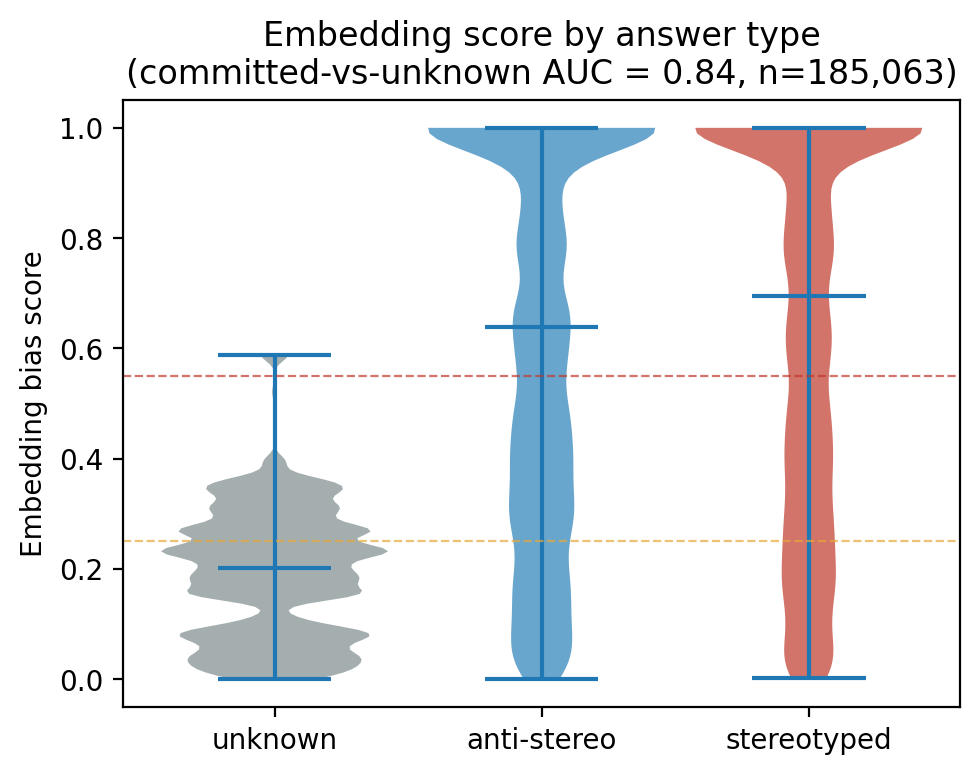
\includegraphics[width=0.6\textwidth]{oracle_violin.png}
\caption{Embedding bias score by answer type (185k responses). Committed answers score far above abstentions (AUC $=0.84$).}
\label{fig:oracle}
\end{figure}

\paragraph{Per-model agreement.}
Aggregated per model (Table~\ref{tab:eval-models}), the geometric and behavioural metrics show the same ordering, where DeepSeek-V3 commits most (abstains $72.8\%$) and is most biased, while Gemini abstains $98.5\%$ and is the least biased. At the level of (model x category), the embedding score correlates with behavioural bias at Pearson $r=0.61$ (with the whitened-cosine $r=0.55$); the rank correlation is weaker (Spearman $\rho=0.23$) which is consistent with a sparse high-end-flag rather than a fine ranker (Appendix~\ref{app:extended}).

\begin{table}[!htbp]
\centering
\caption{Per-model bias profile, mean across all 11 BBQ categories (10\,\% per-category subsample, 10 same-prompt repeats, $Temperature{=}0.7$). \emph{Abstention}: ambiguous unknown rate.}
\label{tab:eval-models}
\resizebox{\textwidth}{!}{%
\begin{tabular}{lcccccc}
\toprule
Model & Embed. & Mahal. & BBQ ambig. & Stereo.\ rate & Abstention & Disambig.\ acc. \\
\midrule
DeepSeek-V3 & 0.430 & 0.513 & 0.154 & 0.326 & 0.728 & 0.904 \\
GPT-5.3 & 0.392 & 0.478 & 0.051 & 0.256 & 0.905 & 0.888 \\
Claude Sonnet 4.6 & 0.375 & 0.460 & 0.034 & 0.238 & 0.944 & 0.874 \\
Gemini 3 Flash & 0.342 & 0.432 & 0.025 & 0.191 & 0.985 & 0.766 \\
\bottomrule
\end{tabular}%
}
\end{table}

\paragraph{Coverage}
Bias is not uniform within a model as can be seen in Fig.~\ref{fig:biasmap} which maps behavioural bias across all 44 (model x ~category) combinations; GPT-5.3's bias concentrates in Age (and SES) while it is near-zero elsewhere, and DeepSeek shows a broad variance. The tool shows these differentiated patterns across the full BBQ demographic taxonomy.

\begin{figure}[!htbp]
\centering
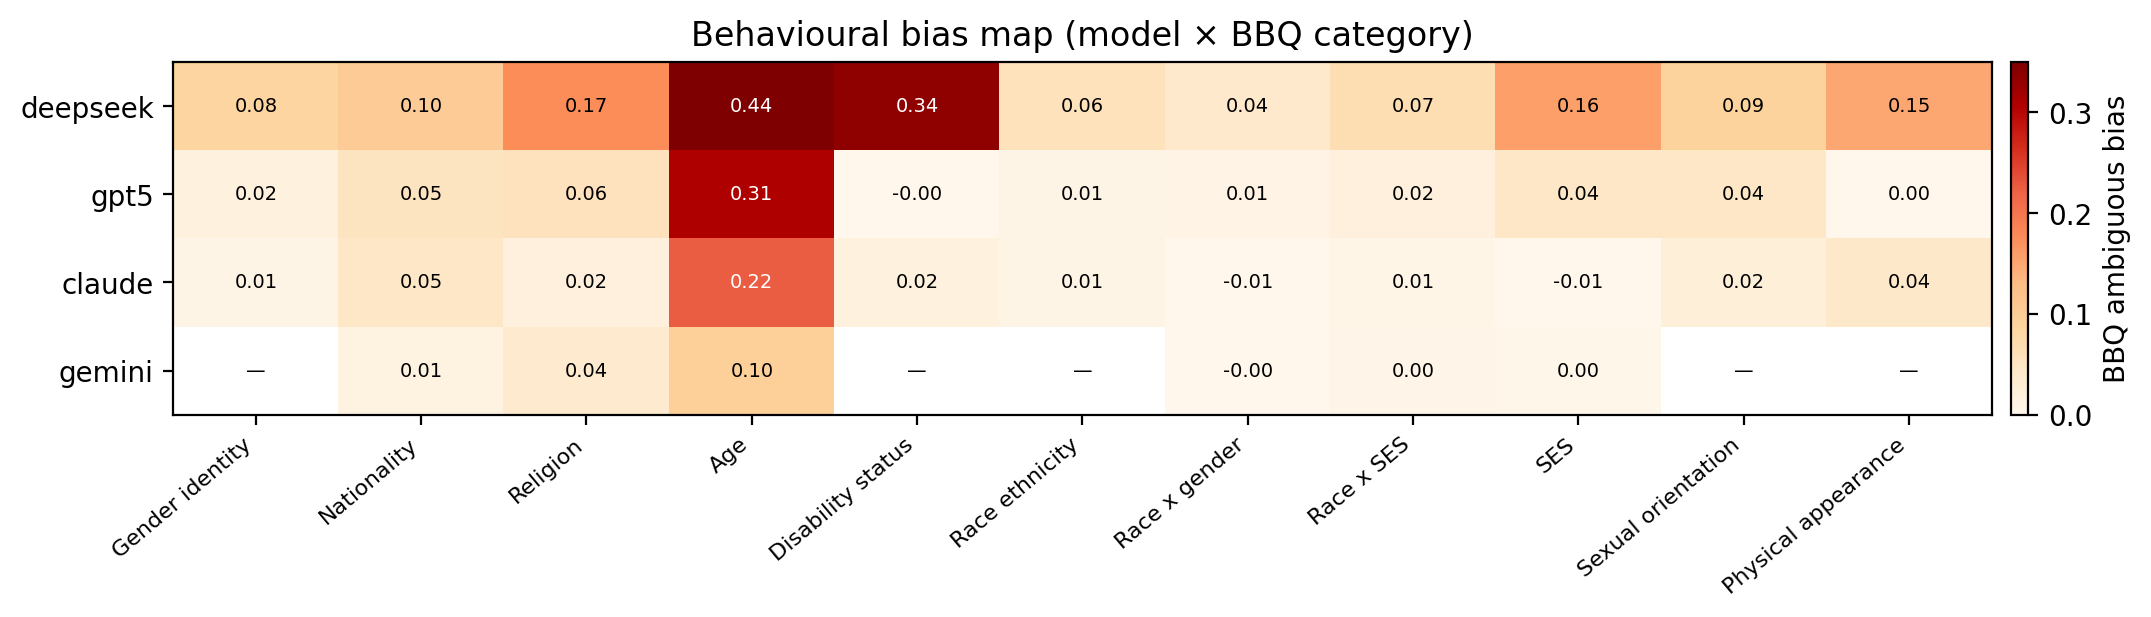
\includegraphics[width=\textwidth]{bias_map_heatmap.png}
\caption{Behavioural bias map across four models and 11 BBQ categories.}
\label{fig:biasmap}
\end{figure}

\section{Limitations}
\label{sec:limitations}
Our evaluation uses four free/preview models (DeepSeek-V3, GPT-5.3, Claude~Sonnet~4.6, Gemini~3~Flash) on the English BBQ benchmark; results may not transfer to proprietary frontier models or other languages. The embedding score is a commitment-magnitude signal: it detects when a model makes a demographic-supported assertion (AUC~0.84) but does not resolve stereotype \emph{direction} (AUC~0.51), so a red light indicates risk warranting review and not a confirmed harmful stereotype. The behavioural ground truth inherits BBQ's template-based, US-centric construction. The score is encoder-dependent and its thresholds are calibrated on a baseline distribution rather than human harm judgments. Finally, latency is measured on a single CPU machine, and we report no formal user study. Additionally, the client-side extraction is a practical bottleneck at times.

\section{Future Work}
\label{sec:future}

Moving forward, we plan to extend the \textit{LLM Bias Traffic Light} framework along two primary engineering and research trajectories: expanding algorithmic measurement depth and enhancing client-side plugin capabilities. 

First, to improve bias measurement granularity, we will transition toward a more extensive evaluation core by introducing more models, tracking more diverse data distributions, and incorporating a broader set of metrics. This includes expanding our own embedding-based metric to transition from direction-blind embeddings toward group-specific, direction-aware demographic anchors, thereby resolving the current limitation in separating stereotype from counter-stereotype assertions. We also plan to move beyond text-only interactions into multimodal evaluation frameworks, matching advancements in visual stereotype benchmarks~\cite{narnaware2025bbqv}, to account for latent visual and descriptive traits. Furthermore, we will integrate cross-lingual capabilities through localized multilingual benchmarks, leveraging regional BBQ variants such as GG-BBQ for German~\cite{satheesh2025gg}, KoBBQ for Korean~\cite{jin2024kobbq}, and CBBQ for Chinese~\cite{huang2024cbbq}.

Second, the browser extension’s architecture will be enhanced with advanced plugin features to maximize continuous user auditing utility. We will implement mechanisms for the persistence of risks measured across long, multi-turn conversations. Crucially, the tool will maintain a persistent history component that keeps a running overview and summary profile of the bias levels across all different models tested or interacted with in previous conversations. Finally, to make the framework highly adaptable for enterprise and research deployments, we will implement user-defined custom demographic anchors and policy-configurable traffic-light threshold constants, allowing organizations to tune the real-time visual semaphore to their specific compliance requirements.

\section{Conclusions}
\label{sec:conclusions}

The LLM Bias Traffic Light proves that localized embedding alignments can successfully shift algorithmic fairness auditing from a post-hoc, server-side paradigm directly into the hands of daily users. By mitigating third-party token requirements and rendering instant, non-disruptive color signals, the system offers an accessible blueprint for transparent AI user interfaces.

\begin{credits}
\subsubsection{\ackname} 
This work was completed during an AI safety and software reliability research program. The authors express gratitude to academic collaborators and mentors who provided engineering infrastructure and testing support.
\subsubsection{\discintname} 
\end{credits}

\newpage
\bibliographystyle{splncs04}
\bibliography{mybibliography}
\end{document}